\documentclass[letterpaper]{article}
\usepackage{aaai}
\usepackage{times}
\usepackage{helvet}
\usepackage{courier}
\usepackage{tikz}
\usepackage{caption}
\usepackage{subcaption}
%\usepackage{pgfplots}

%\pgfplotsset{width=10cm,compat=1.9}
%\usepgfplotslibrary{external}
%\usetikzlibrary{patterns}
%\tikzexternalize
%\listfiles


\setlength{\pdfpagewidth}{8.5in}
\setlength{\pdfpageheight}{11in}
\pdfinfo{
/Title (Minimal Matching for an Autonomous Car Sharing System)
/Author (Anonymous)}
\setcounter{secnumdepth}{0}  
\begin{document}
% The file aaai.sty is the style file for AAAI Press 
% proceedings, working notes, and technical reports.
%
\title{On Optimizing the User-Vehicle Assignment for an Autonomous Car Sharing System}
\author{Anonymous}
\maketitle
\begin{abstract}
\begin{quote}
We seek to improve the performance of a fleet of shared autonomous vehicles through improved matching of vehicles to passengers requesting rides. Carsharing programs provide an alternative to private vehicle ownership. Combining carsharing programs with autonomous vehicles would improve user access to vehicles which removes one of the main challenges these programs face for widescale adoption. While the ability to easily move cars to meet demand would be significant for carsharing programs it could lead to worse system performance if the assignment of cars to users is not done in an intelligent way. In this paper we consider car sharing with autonomous vehicles as an assignment problem and examine different methods for matching cars to users to meet different criteria. We show how applying a recent algorithm for minimizing the maximal edge in a perfect matching can result in a more efficient and reliable carsharing system. Our results also highlight some of the problems with greedy or decentralized approaches.
\end{quote}
\end{abstract}

\noindent 

\section{Introduction}
Autonomous vehicle technology is becoming a reality. Driverless cars have the potential to make travel safer, increase fuel economy, and reduce pollution (need citation). However the potential of this technology does not have to be limited to a new way to move people from point A to point B. Autonomous vehicles have the potential to revolutionize modern transportation systems (cite some AIM related work). One such system is carsharing.

Carsharing is a transportation service where users can access a personal vehicle when desired without the need to own a private vehicle. A user reserves a vehicle to use as a private vehicle. Service begins at designated car parking spots and must end at one of these spots. Current systems such as Car2Go or ZipCar have car parking spots scattered throughout the city to give users flexibility in trip origin and destinations. One problem with current systems is that vehicles may be moved from high demand to low demand areas. Then the vehicle is likely to remain unused for a long time before being used again. Additionally, users may not desire to walk to an access point or walk from a dropoff location to their final destination. Both of these problems have hindered the growth of carsharing programs.

Autonomous vehicles offer a promising solution to these problems. An autonomous vehicle can meet a user at a requested position and drop them off at the user's desired destination. When not in use, the vehicle can move to other users or strategically relocate to an area with high demand \cite{fagnant2014travel}. Driverless cars can remain in service at all times (except for service or refueling) so the carsharing fleet remains close to full size throughout the day. And automated communication between cars can allow for coordination to improve system performance. This paper considers carsharing with autonomous vehicles as a multi-agent system and looks at how to best coordinate the assignment of vehicles to users to improve the system performance. Specifically we view users and available vehicles as forming a bipartite graph. Then different maximal matching algorithms can be applied and their effects evaluated.

For an autonomous carsharing system to be used it needs to provide users service in the shortest amount of time possible after they request a ride. Miles traveled without passengers in the vehicle should be minimized as they are not directly serving trips but still contribute to pollution and add fuel costs. This suggests that a simple minimum cost maximal matching of the user-vehicle graph could meet both of these objectives. However, in the context of carsharing, there are two additional criteria. The system should not give some users fast service at the expense of long waits for others. And the system must be reliable so we want all trips to be served and to have a low variance over wait time. To better address these issues we use an algorithm called SCRAM from the class of minimal-makespan matching algorithms \cite{macalpine2015scram}. SCRAM finds a matching in a bipartite graph such that the maximal cost edge in the matching is minimized. 

This paper is laid out as follows: Section 1 describes the agent-based model we use to simulate carsharing. Section 2 introduces different algorithms and explains their advantages in a carsharing system. Section 3 presents and discusses results and Section 4 proposes future work and concludes.


\section{Car Sharing Model}

% Basic overview
For experiments we use the agent-based car sharing model proposed by Fagnant and Kockelman \cite{fagnant2014travel}. This model represents a 10 mile by 10 mile city as a grid of 0.25 mile by 0.25 mile grid cells. Vehicles can can move north, south, east, or west to adjacent cells. Motion within the cells is not modeled. Diagonal motion is not permitted and cars do not interfere with each other's path. Time is discretized into five minute intervals for a total of 288 time steps per day. Each run of the simulation corresponds to one 24 hour day.

% Trip Generation
Users requesting trips are generated in each grid cell according to a rate that decreases the farther a cell is from the city center. This rate is the mean for a Poisson process from which a number of trips is drawn for the corresponding cell. The distance and start time for each trip is drawn from a distribution based on U.S. National Highway Traffic Safety Administration trip distance data. While all trips for the day are generated at the start of the run, requests for rides are not made until the start time of the trip. 

% Simulation Cycle
At each time step available vehicles are matched to users requesting trips. If a user cannot be served they are added to a wait list and can request a ride again at the next time step. If a user cannot be served after 30 minutes of wait time the trip is considered unserved. Vehicles that could not serve trips because they were low on fuel go to the nearest fueling station (assumed to be within the same grid cell) and are out of service for two time steps (10 minutes). Then vehicles move to the passengers. Vehicles already with passengers proceed to their trip destination. Each vehicle can move a fixed number of grid cells depending on the current maximum speed.

% Fleet Size
We consider two schemes for determining the number of cars that are needed to provide adequate service. As in \cite{fagnant2014travel}, the number of cars can be determined by running the simulation for 20 runs with each run initialized with zero cars. The simulation cycle proceeds normally except after a trip has waited for 10 minutes a new car is generated at the start location of the trip. The number of cars generated is an estimate of the required fleet size. The average number of cars generated across these 20 runs is the fleet size. A final run repeats this procedure until the correct fleet size has been generated. Alternatively, since we wish to compare the sensitivity of different methods to variations in the fleet size, we can specify a fixed number of vehicles. In this case the above procedure can be repeated until the requested fleet size is reached and then no more cars are generated.

% Limitations
This model approximates the effects of a car sharing system in a 10 mile by 10 mile urban area. Car speed has small variations due to time of day and distance from the city center but is otherwise fairly constant. The simulation only models vehicles and passengers using the car sharing service. The presence of other modes of transportation is reflected in the trip generation rates and speed variations but these are only approximations. Nonetheless the model has been used in other car sharing studies \cite{fagnant2015operations} to date and is realistic enough for the purpose of this work. 

\section{Matching Algorithms}

Using the described carsharing model we want to determine how the assignment of vehicles to users affects the performance of the system. An easy way to handle the assignment problem would be to let users request the nearest vehicle to them on a first come first served basis. Unfortunately such simple approaches are not likely to be optimal in terms of the amount of waiting that users have or the number of trips that can be served. In addition, we would like to have a fair system in which some users are not waiting for long periods of time so that other users do not have to wait as long.

\begin{figure}
\centering
\begin{subfigure}[t]{0.2\textwidth}
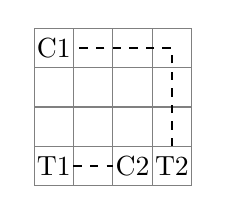
\begin{tikzpicture}
\centering
\draw[step=0.5cm,color=gray] (-1,-1) grid (1,1);
\node at (-0.75,+0.75) {C1};
\node at (-0.75,-0.75) {T1};
\node at (+0.25,-0.75) {C2};
\draw [dashed,thick] (-0.5,-0.75) -- (0,-0.75);
\draw [dashed,thick] (0.75,-0.5) -- (0.75,0.75) -- (-0.5,0.75);
\node at (+0.75,-0.75) {T2};
\end{tikzpicture}
        \caption{Decentralized}
\end{subfigure}
~
\begin{subfigure}[t]{0.2\textwidth}
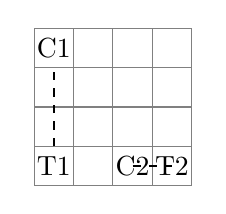
\begin{tikzpicture}
\centering
\draw[step=0.5cm,color=gray] (-1,-1) grid (1,1);
\node at (-0.75,+0.75) {C1};
\node at (-0.75,-0.75) {T1};
\node at (+0.25,-0.75) {C2};
\draw [dashed,thick] (-0.75,-0.5) -- (-0.75,0.5);
\draw [dashed,thick] (0.25,-0.75) -- (0.75,-0.75);
\node at (+0.75,-0.75) {T2};
\end{tikzpicture}
\caption{Greedy}
\end{subfigure}
~
\begin{subfigure}[t]{0.2\textwidth}
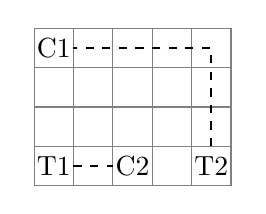
\begin{tikzpicture}
\draw[step=0.5cm,color=gray] (-1,-1) grid (1.5,1);
\node at (-0.75,+0.75) {C1};
\node at (-0.75,-0.75) {T1};
\node at (+0.25,-0.75) {C2};
\draw [dashed,thick] (-0.5,-0.75) -- (0,-0.75);
\draw [dashed,thick] (1.25,-0.5) -- (1.25,0.75) -- (-0.5,0.75);
\node at (+1.25,-0.75) {T2};
\end{tikzpicture}
\caption{Greedy}
\end{subfigure}
~
\begin{subfigure}[t]{0.2\textwidth}
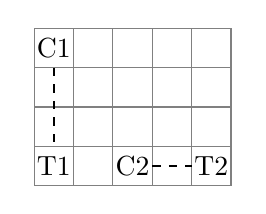
\begin{tikzpicture}
\draw[step=0.5cm,color=gray] (-1,-1) grid (1.5,1);
\node at (-0.75,+0.75) {C1};
\node at (-0.75,-0.75) {T1};
\node at (+0.25,-0.75) {C2};
\draw [dashed,thick] (0.5,-0.75) -- (1.0,-0.75);
\draw [dashed,thick] (-0.75,0.5) -- (-0.75,-0.5);
\node at (+1.25,-0.75) {T2};
\end{tikzpicture}
\caption{Hungarian}
\end{subfigure}
~
\begin{subfigure}[t]{0.2\textwidth}
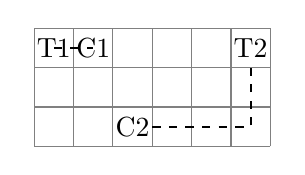
\begin{tikzpicture}
\centering
\draw[step=0.5cm,color=gray] (-1.5,-0.5) grid (1.5,1.0);
\node at (-0.75,+0.75) {C1};
\node at (-1.25,+0.75) {T1};
\node at (-0.25,-0.25) {C2};
%\draw (-0.25,-0.75) ellipse (8mm and 3mm);
\draw[dashed,thick] (-1.25,0.75) -- (-.75,0.75);
\draw[dashed,thick] (0,-0.25) -- (1.25,-0.25) -- (1.25,0.5);
\node at (+1.25,+0.75) {T2};
\end{tikzpicture}
\caption{Hungarian}
\end{subfigure}
~
\begin{subfigure}[t]{0.2\textwidth}
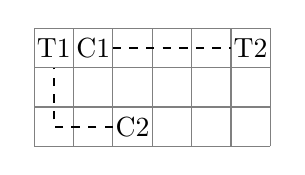
\begin{tikzpicture}
\centering
\draw[step=0.5cm,color=gray] (-1.5,-0.5) grid (1.5,1.0);
\node at (-0.75,+0.75) {C1};
\node at (-1.25,+0.75) {T1};
\node at (-0.25,-0.25) {C2};
%\draw (-0.25,-0.75) ellipse (8mm and 3mm);
\draw[dashed,thick] (-0.5,0.75) -- (1,0.75);
\draw[dashed,thick] (-0.5,-0.25) -- (-1.25,-0.25) -- (-1.25,0.5);
\node at (+1.25,+0.75) {T2};
\end{tikzpicture}
\caption{Scram}
\end{subfigure}
\label{smallExampleFigure}
\caption{These small examples illustrate some of the disadvantages of the different algorithms used in the experiments. For a fixed scenario along each row, the drawings on the left show a suboptimal solution with one algorithm and the drawings on the right show a better solution from a different algorithm. The bottom row shows how Scram minimizes the longest distance traveled but not the total distance traveled.}
\end{figure}

\paragraph{Decentralized Greedy Matching}
Without a centralized trip-car assignment system trips would need to request the nearest vehicle, similar to how users of Uber or Lyft look for nearby vehicles. This decentralized method can be implemented as a greedy matching of trips to vehicles. In a random order, trips are assigned to the closest vehicle to them. If one is not available they are added to a wait list and will make requests at the next time step. We assume that passengers can request a vehicle from anywhere in the city. In practice this might be constrained to a local area to prevent cars from having to cross the entire city to reach a passenger. This would result in some passengers not receiving service due to no cars in the area. Figure \ref{exampleFigure} illustrates how this approach can result in inefficiencies.


\paragraph{Centralized Greedy Matching}
To improve on the decentralized greedy approach we consider a centralized greedy approach. Each trip looks for a car within a one cell radius of itself. After all trips have made this search the radius is increased and trips search again. The advantage of this approach is that a vehicle will not be assigned to a passenger if it could have served another passenger in less time. The disadvantage is that there are no guarantees that the assignment will be optimal. Figure \ref{exampleFigure} gives a scenario where this approach fails to produce the optimal solution.

This radius can either increase up to searching the entire city or terminate at a fixed limit (e.g. the distance a vehicle can travel in one time step).

\paragraph{Hungarian Algorithm}
A natural improvement is the Hungarian algorithm \cite{kuhn1955hungarian} which finds a minimum cost perfect matching in a bipartite graph. The Hungarian algorithm can be implemented to run in time $O(n^3)$ which is fast enough to compute our car to passenger assignment in a few seconds. The input to the algorithm is a set of $n$ cars and $n$ trips and a distance metric to be minimized. Since we have an input of $n$ cars and $m$ trips we can create $|n-m|$ dummy passengers if $n > m$ or dummy cars if $m > n$. Setting the distance to a dummy car/passenger to zero results in the Hungarian algorithm returning the minimized distance for unequal $m$ and $n$ \cite{macalpine2015scram}.

\paragraph{Minimal Makespan Matching}
The Hungarian algorithm produces a minimum cost perfect matching but the optimal solution does not consider fairness of the system. In our scenario this equates to the possibility that some trips have a much longer wait time even though the total wait across all trips is minimized. To improve on this we use a scalable collision-avoiding role assignment with minimal-makespan (SCRAM) algorithm to find an assignment that minimizes the longest distance that any vehicle must travel to a passenger. Specifically we implement the Minimum Maximal Distance + Minimum Sum Distance$^2$ (MMD+MSD$^2$) proposed in \cite{macalpine2015scram}. Given a bipartite graph, $G = ({S,T},E)$  this algorithm first finds the minimum maximal edge in a perfect matching from $S$ to $T$. Then edges in $E$ with length larger than this edge are removed from the edge set. Finally, the Hungarian algorithm is ran on this reduced set of edges to find the minimum cost matching.  

\section{Experimental Setup}
To compare different approaches we run two sets of experiments. The first set of experiments compares the performance of the above algorithms over 100 consecutive days of fleet use. Since each the events of each day affect the next, multiple days are needed to get an idea of system performance. In these experiments the fleet size is set to 1000 vehicles which was experimentally found to be able to serve all users with any method of assignment. It is important that all trips be served in order to make meaningful comparisons. This is because an assignment strategy could reduce average wait time by simply not serving passengers that would have to wait a long time. We run 50 trials of 100 days each for each method of assignment.

The second set of experiments compares the ability of different methods to serve trips with different fleet size. Starting at a fleet size of 500 vehicles, fleet size is increased in increments of 100 and each method is ran for 100 days with each fleet size.

\section{Results}

This section presents and discusses the experimental results. Statistical significance is computed using a t-test for all results.

\subsection{Unoccupied Miles Traveled}

The first comparison we make is on the average amount of unoccupied vehicle miles per day. Unoccupied miles are necessary to reach passengers but also mean extra fuel costs and wear on vehicles that does not directly contribute to serving a trip. Figure \ref{unoccupiedGraph} shows the amount of miles traveled by vehicles with no passengers in them. The results show that both of the more sophisticated matching approaches are able to reduce this number by approximately 20 percent from the baseline approach. The Hungarian algorithm performs better than SCRAM. This is because the Hungarian algorithm is focused on minimizing the total while SCRAM spreads out the travel.  

\begin{figure}
%\resizebox {\columnwidth} {!} {
%\begin{tikzpicture}
%\begin{axis}[
%	x tick label style={
%	/pgf/number format/1000 sep=},
%	ylabel=Average Unoccupied Distance (miles per day),
	%symbolic x coords={0,Decentralized,Greedy,Hungarian,SCRAM},
  %  xtick=data,
 %   enlarge y limits=0.01,
%	enlarge x limits=0.15,
%	legend style={at={(0.5,-0.1)},
	%anchor=north,legend columns=-1},
  %  ybar = 3pt,
 %   bar width=20pt
%]
%\addplot [fill=blue,error bars/.cd, y dir=both, y explicit,]
%	coordinates {(Decentralized,18524.0803) += (0,31.4938344758) -= (0,31.4938344758) (Greedy,15479.34128) += (0,13.6964034878) -= (0,13.6964034878)
%		 (SCRAM,14605.7718336) += (0,15.4548969092) -= (0,15.4548969092) (Hungarian,14344.3014) += (0,14.9256398871) -= (0,14.9256398871)};

%\end{axis}
%\end{tikzpicture}
%}
\label{unoccupiedGraph}
\caption{This bar graph shows how different assignment methods result in different amounts of unoccupied travel. Error bars are for a 95$\%$ confidence level.}
\end{figure}

\subsection{Passenger Wait Time}

The next point of comparison is passenger wait time. Wait time is a combination of how long it takes users to be matched to a vehicle and how long it takes for the assigned vehicle to reach the user:
$$Wait_{total} = Wait_{matching} + Wait_{travel} $$
. For all methods the average wait was less than five minutes (i.e. on average all users could be assigned a vehicle the first time they requested one) which means the first term will be zero for most trips. This means that the average wait time is highly correlated with unoccupied miles traveled. 

While a minimal average wait time is good, we also want the service to be reliable and predictable for all of the users. To characterize this, we look at variance in the wait time and the number of users that have to wait longer than certain time thresholds. Results are shown in Figure \ref{averageWaitVarianceGraph} and Figure \ref{averageWaitTimes}.

(SCRAM results place holder for variance)

Figure \ref{averageWaitTimes} shows that SCRAM is able to minimize the number of trips that must wait longer than each threshold. This comes from SCRAM's minimal-makespan property. SCRAM's solution has a slightly longer average wait than the Hungarian algorithm but less users are having longer waits. Unreliable service or long wait times are likely to cause users to abandon carsharing for more reliable sources of transportation such as private vehicles. If the system loses users it will lose revenue which may further decrease its capacities. This is why reliable service must be provided to all users.

\begin{figure}
%\resizebox {\columnwidth} {!} {
%\begin{tikzpicture}
%\begin{axis}[
%	x tick label style={
%	/pgf/number format/1000 sep=},
%	ylabel=Average Wait Time Variance,
%	symbolic x coords={0,Decentralized,Greedy,Hungarian,SCRAM},
%    xtick=data,
 %   enlarge y limits=0.01,
%	enlarge x limits=0.15,
%	legend style={at={(0.5,-0.1)},
%	anchor=north,legend columns=-1},
%	ybar interval=0.5,
 %   ybar = 3pt,
%    bar width=20pt
%]
%\addplot [fill=red, error bars/.cd, y dir=both, y explicit]
%	coordinates {(Decentralized,0) += (0,0) -= (0,0) (Greedy,0)
%		 (SCRAM,0) (Hungarian,0)};

%\end{axis}
%\end{tikzpicture}
%}
\label{averageWaitVarianceGraph}
\caption{This bar graph shows how different assignment methods result in different amounts of variance within travel time. Error bars are for a 95$\%$ confidence level.}
\end{figure}

\begin{figure}
%\resizebox {\columnwidth} {!} {
%\begin{tikzpicture}
%\begin{axis}[
%	x tick label style={
%	/pgf/string format/1000 sep=0pt anchor=east shift=-4pt},
%	ylabel=Number of passengers,
%	symbolic x coords={0,Five,Ten,Fifteen,D},
%    xtick=data,
%    enlarge y limits=0.01,
%	enlarge x limits=0.15,
%	legend style={at={(0.5,-0.1)},
%	anchor=north,legend columns=-1},
%	ybar interval=0.7,
%    ybar = 1pt,
%    bar width=15pt
%]
%Decentralized
%\addplot [pattern=north east lines,error bars/.cd, y dir=both, y explicit,]
%	coordinates {(Five,2071.4542) += (0,14.3062459029) -= (0,14.3062459029) (Ten,390.5364) %+= (0,3.1325882223) -= (0,3.1325882223)
%		 (Fifteen,130.0746) += (0,1.5169568583) -= (0,1.5169568583)};

%Greedy
%\addplot [pattern=dots, error bars/.cd, y dir=both, y explicit,]
%	coordinates {(Five,1623.7748) += (0,4.4938187306) -= (0,4.4938187306) (Ten,353.9534) %+= (0,1.8198260124) -= (0,1.8198260124)
%		 (Fifteen,78.5602) += (0,0.7429254263) -= (0,0.7429254263)};

%Hungarian		 
%\addplot [pattern=crosshatch, error bars/.cd, y dir=both, y explicit,]
%	coordinates {(Five,974.4834) += (0,3.9463704624) -= (0,3.9463704624) (Ten,118.404) += %(0,0.95148793) -= (0,0.95148793)
%		 (Fifteen,24.9586) += (0,0.4115085269) -= (0,0.4115085269)};

%SCRAM		 
%\addplot [pattern=north west lines,error bars/.cd, y dir=both, y explicit,]
%	coordinates {(Five,840.765467247) += (0,4.5148281834) -= (0,4.5148281834) %(Ten,26.095930545) += (0,0.5505090487) -= (0,0.5505090487)
%		 (Fifteen,4.8304617135) += (0,0.1088751011) -= (0,0.1088751011)};

%\end{axis}
%\end{tikzpicture}
%}
\label{averageWaitTimes}
\caption{This bar graph shows how different algorithms can match more of the trips sooner. Error bars are for a 95$\%$ confidence level.}
\end{figure}

\subsection{Sensitivity of Methods to Fleet Size}

\begin{figure}
%\resizebox {\columnwidth} {!} {
%\begin{tikzpicture}
%\begin{axis}[
%	xlabel=Fleet Size,
%	ylabel=Number of Unserved Trips]
%\addplot[color=blue,mark=x, error bars/.cd, y dir=both, y explicit,] coordinates {
%	(500,    100)
%	(600,   90)
%	(700,   80)
%	(800,  70)
%	(900,  60)
%	(1000,  50)
%};

%\addplot[color=blue,mark=x,error bars/.cd, y dir=both, y explicit,] coordinates {
%	(500,    90)
%	(600,   80)
%	(700,   70)
%	(800,  60)
%	(900,  50)
%	(1000,  40)
%};

%\addplot[color=red,mark=*,error bars/.cd, y dir=both, y explicit,] coordinates {
%	(500,    80)
%	(600,   70)
%	(700,   60)
%	(800,  50)
%	(900,  40)
%	(1000,  30)
%};

%\addplot[color=red,mark=*,error bars/.cd, y dir=both, y explicit,] coordinates {
%	(500,    70)
%	(600,   60)
%	(700,   50)
%	(800,  40)
%	(900,  30)
%	(1000,  20)
%};
	

%\legend{Decentralized, Greedy, Hungarian, SCRAM}
%\end{axis}
%\end{tikzpicture}
%}
\label{fleetSizeGraph}
\caption{How fleet size affects the number of vehicles that can be served.}
\end{figure}

\section{Conclusion and Future Work}

We have presented a comparison of different methods for assigning vehicles to users for a carsharing system using autonomous vehicles. Our experiments show that employing an optimal perfect matching algorithm can improve performance of a system in terms of wasted travel and customer service.

The current approach is short sighted in that it only considers vehicles available at the time of assignment. Any of the assignment methods could be adapted to consider vehicles that will soon be available. This could be done by representing the vehicles distance to a passenger as the distance from the passenger to the vehicle destination plus the vehicles remaining distance to travel. In situations where the fleet size is limited this could allow the system to directly tell users if it will be possible to serve them and how long they have to wait. Another potential direction is ridesharing which may reduce to a vehicle routing problem.

\bibliography{CarSharing}
\bibliographystyle{aaai}
\end{document}
